\documentclass[conference]{IEEEtran}
\IEEEoverridecommandlockouts
\usepackage{cite}
\usepackage{amsmath,amssymb,amsfonts}
\usepackage{algorithmic}
\usepackage{graphicx}
\usepackage{textcomp}
\usepackage{xcolor}
\usepackage{booktabs}
\usepackage{subcaption}
\usepackage{multirow}
\usepackage{placeins}
\graphicspath{{images/}}
\def\BibTeX{{\rm B\kern-.05em{\sc i\kern-.025em b}\kern-.08em
    T\kern-.1667em\lower.7ex\hbox{E}\kern-.125emX}}

\begin{document}

\title{When DQN Breaks: Diagnosing Flat-MLP Collapse in UAV--LoRaWAN Data Collection and Fixing It with Relational RL}

\author{
\IEEEauthorblockN{Atilade Gabriel Oke}
\IEEEauthorblockA{
\textit{Department of Electrical and Electronic Engineering}\\
\textit{The University of Manchester}\\
Manchester, United Kingdom\\
atilade.oke@student.manchester.ac.uk}
}

\maketitle

\begin{abstract}
UAV-assisted LoRaWAN data collection requires a flight policy that generalises across sensor densities and deployment areas without retraining. We train a Deep Q-Network (DQN) with Domain Randomisation and Curriculum Learning, then test it systematically across five co-scaled conditions. The DQN reaches 99.4\% sensor coverage at $200{\times}200$~m with 20~sensors, then drops to 52.7\% at $300{\times}300$~m with 30~sensors and 27.5\% at $400{\times}400$~m with 40~sensors, falling below both greedy baselines at every condition beyond $N{=}20$. Trajectory analysis shows the UAV spends 100\% of its timesteps on boundary cells regardless of reward penalties. The fault is structural: the flat MLP input concatenates per-sensor features at fixed array positions, coupling sensor identity to array index. When Domain Randomisation changes sensor layouts across episodes, that coupling breaks generalisation. We replace the flat MLP with a cross-attention module where the UAV embedding queries a set of sensor tokens. The attention mask handles variable sensor counts transparently and the output does not change when sensors are reordered. Trained with PPO under the same curriculum, this Relational RL agent reaches 97.7\% coverage at $300{\times}300$/30~sensors, 76.5\% at $400{\times}400$/40~sensors, and leads every non-oracle agent at all five conditions. Against a TSP Oracle upper bound the Relational agent recovers 73--98\% of oracle coverage across the range, degrading because of battery budget rather than policy failure.
\end{abstract}

\begin{IEEEkeywords}
UAV, LoRaWAN, deep reinforcement learning, attention, permutation invariance, domain randomisation, age of information, SF monoculture
\end{IEEEkeywords}

% ============================================================
\section{Introduction}
% ============================================================

Equipping UAVs with LoRaWAN gateways gives IoT deployments wide coverage at low infrastructure cost~\cite{wei2022uav,zeng2016wireless,mozaffari2019tutorial}. The catch is that a moving gateway shifts the link quality seen by every sensor at once. Standard Adaptive Data Rate (ADR) responds by pushing sensors toward the same Spreading Factor (SF), which collapses the concurrent channel capacity that makes LoRa worth using~\cite{zorbas2025revisiting,bor2016lora,augustin2016lora}. A policy that treats UAV position as an active ADR control input can prevent this SF Monoculture~\cite{zorbas2025revisiting,xiong2023flyinglora}.

We trained a DQN~\cite{mnih2015humanlevel} with Domain Randomisation (DR)~\cite{tobin2017domain} and Curriculum Learning (CL)~\cite{bengio2009curriculum}. At small scale it works: at $200{\times}200$~m with 20~sensors the agent reaches 99.4\% sensor coverage (NDR) and the training curve is stable across all three curriculum stages. At larger conditions it fails. At $300{\times}300$~m with 30~sensors NDR drops to 52.7\%, which is 32 percentage points below the SF-Aware Greedy baseline. At $400{\times}400$~m with 40~sensors it falls further to 27.5\%. The UAV physically can explore the grid and the reward penalises boundary stays, yet the agent patrols the perimeter and never enters the interior.

We traced the failure to the input representation. The flat MLP concatenates sensor features in a fixed order, so sensor~$i$ always occupies positions $3{+}5(i{-}1)$ to $3{+}5i{-}1$ in the input vector. The policy is permutation-dependent: it has learned that ``the sensor at array index~3 is roughly here in the grid.'' When DR randomises sensor positions across episodes, that implicit mapping breaks. At small scale the model partially memorises position statistics. At larger scale the distribution is too broad and the policy degrades to a boundary patrol that ignores interior sensors.

The fix is a permutation-invariant architecture. Work on relational inductive biases in RL~\cite{zambaldi2018relational} and on set-function approximation~\cite{zaheer2017deepsets} shows that attention-based networks generalise better to combinatorial inputs than fixed-size MLPs. We built a cross-attention module~\cite{vaswani2017attention}: the UAV state is a query token; each sensor produces a key-value token; multi-head attention aggregates sensor context with a padding mask for unused slots. Trained with PPO~\cite{schulman2017proximal} on the same schedule, this Relational RL agent restores coverage without any changes to the environment, reward, or training budget.

The contributions of this paper are:
\begin{itemize}
    \item A Gymnasium-compatible~\cite{towers2024gymnasium} LoRaWAN simulation with Two-Ray propagation~\cite{rappaport2002wireless}, log-normal shadowing, EMA-based ADR~\cite{slabicki2018adaptive,augustin2016lora}, and Capture-Effect collision resolution~\cite{croce2020lora,reynders2016range}.
    \item A DQN with DR and CL, together with a rigorous 50-seed demonstration of where and why it breaks.
    \item A diagnosis of the failure as permutation-dependent flat-MLP encoding, supported by boundary-occupancy diagnostics.
    \item A Relational RL agent with masked cross-attention that is permutation-invariant by construction and restores scalability across all tested conditions.
    \item A 50-seed evaluation across five co-scaled conditions against two greedy baselines and a TSP Oracle upper bound.
\end{itemize}

% ============================================================
\section{Related Work}
% ============================================================

\subsection{UAV data collection via DRL}

Bayerlein et al.~\cite{bayerlein2020uav} train a DDQN to collect data from IoT sensors in urban environments using a UAV-position-centred map input, and find that a centred representation outperforms a global one as scenario parameters vary. This is consistent with our result: fixed sensor-index encoding breaks as layout diversity grows. Liu et al.~\cite{liu2019uav} and Nemer et al.~\cite{nemer2022energyefficient} apply DRL to energy-efficient UAV coverage and optimise Jain's fairness~\cite{jain1984quantitative} alongside throughput, but both use small fixed-layout scenarios that sidestep the scaling problem. Zhang et al.~\cite{zhang2021energy} confirm that hovering costs more power than translational flight in rotary-wing platforms, motivating our hover penalty. Li et al.~\cite{li2020uav} survey UAV communications for 5G and Zeng and Zhang~\cite{zeng2017energy} establish trajectory optimisation baselines. Al-Hourani et al.~\cite{alhourani2014optimal} derive the optimal UAV altitude for LoS coverage probability; we fix altitude at 100~m and optimise horizontal trajectory only.

\subsection{LoRaWAN protocol and the SF Monoculture}

Zorbas et al.~\cite{zorbas2025revisiting} provide the clearest formal analysis of SF-allocation convergence under standard ADR and recommend RL as the remedy. FlyingLoRa~\cite{xiong2023flyinglora} is the closest prior system: it plans energy-efficient LoRa paths but treats the protocol as a static constraint. We let the trajectory actively manage ADR state instead. Croce et al.~\cite{croce2020lora} characterise the Capture Effect that makes co-SF collision resolution non-trivial; the SNR-based SF thresholds we use (Table~\ref{tab:sf}) follow from their measurements. The EMA-ADR model follows~\cite{slabicki2018adaptive,augustin2016lora}; Two-Ray propagation follows~\cite{rappaport2002wireless,alhourani2014optimal}. Lee et al.~\cite{lee2025quasi} address multi-UAV coordination via Quasi-Distributed DQL; their architecture is compatible with our single-UAV policy as a base agent. Ahmed et al.~\cite{ahmed2026marl} propose a MAPPO framework for joint SF, bandwidth, and transmission-power allocation across multiple flying LoRa gateways.

\subsection{Permutation-invariant policies}

Zaheer et al.~\cite{zaheer2017deepsets} prove that any permutation-invariant function over a set decomposes into per-element functions followed by a global aggregator. Vaswani et al.~\cite{vaswani2017attention} give a practical realisation via multi-head attention with richer inter-element interactions. Zambaldi et al.~\cite{zambaldi2018relational} apply self-attention to RL and show gains on combinatorial reasoning tasks. Kool et al.~\cite{kool2019attention} use cross-attention to build a competitive TSP solver, which is the combinatorial structure underlying our Oracle baseline. Cappart et al.~\cite{cappart2023combinatorial} survey graph neural networks for combinatorial optimisation more broadly. Our architecture applies these ideas to the UAV routing problem, where the active sensor set is an unordered input.

\subsection{Training methodology}

Bengio et al.~\cite{bengio2009curriculum} introduced curriculum learning as a training schedule over increasingly difficult examples. Tobin et al.~\cite{tobin2017domain} showed that DR over simulation parameters can produce policies that transfer without retraining. OpenAI~\cite{openai2019dexterous} combined both for robotic manipulation. Matiisen et al.~\cite{matiisen2017teacher} proposed teacher-student curriculum scheduling that informs our per-stage competence gates. Zhao et al.~\cite{zhao2021sim2real} survey the sim-to-real gap; Luong et al.~\cite{luong2019drl} survey DRL applications in wireless communications. The transformer-in-RL landscape is covered by~\cite{chen2021decision,parisotto2020gtrxl}; Schulman et al.~\cite{schulman2016gae} introduce the Generalised Advantage Estimation used in PPO training. The DQN implementation uses Stable-Baselines3~\cite{raffin2021stable}; the Relational RL agent uses Ray RLlib.

% ============================================================
\section{System Model}
% ============================================================

We consider $N$ static LoRa sensors uniformly distributed over a square grid of side $L$~m. Each sensor generates monitoring data at a Poisson rate, accumulating in a buffer of capacity $B_{\max}{=}1{,}000$~bytes. A rotary-wing UAV acts as a mobile LoRaWAN gateway over a mission of $T{=}2{,}100$ discrete timesteps. The system is illustrated in Fig.~\ref{fig:sysmodel}.

\begin{figure}[htbp]
    \centering
    \includegraphics[width=\columnwidth]{uav}
    \caption{System model: a single UAV gateway at 100~m altitude collects uplink data from $N$ IoT sensors over a grid of side $L$~m. LoRa links operate under EMA-based ADR (SF7--SF12), log-normal shadowing, and Capture-Effect collision resolution.}
    \label{fig:sysmodel}
\end{figure}

\subsection{UAV kinematics and energy}

The UAV operates at fixed altitude $h{=}100$~m with five discrete actions: move North, South, East, West (each 10~m per step at 10~m/s), or Hover. Battery energy evolves as:
\begin{equation}
E_{k+1} = E_k - P(a_k) \cdot \Delta t
\label{eq:battery}
\end{equation}
where $P(\text{Hover}){=}700$~W and $P(\text{move}){=}500$~W. Hovering costs more power than translational flight in rotary-wing platforms because it requires continuous thrust against gravity with no translational lift~\cite{zhang2021energy,zeng2017energy}. The model parameters are taken from the DJI TB60 (274~Wh capacity).

\subsection{Channel model}

We use the Two-Ray Ground Reflection model~\cite{rappaport2002wireless}, which captures the constructive and destructive interference effects of ground reflections at low UAV altitudes:
\begin{equation}
P_r = P_t G_t G_r \frac{h_t^2 h_r^2}{d_{i,t}^4}
\label{eq:tworay}
\end{equation}
where $h_t$ is sensor height, $h_r{=}100$~m is UAV altitude, and $d_{i,t}$ is 3D slant range. The quartic $1/d^4$ decay applies beyond the breakpoint $d_{\text{break}} = 4\pi h_t h_r / \lambda \approx 1{,}160$~m; free-space loss applies below it. Log-normal shadowing $X_\sigma \sim \mathcal{N}(0,4~\text{dB})$ is added to represent physical obstructions~\cite{alhourani2014optimal}. The received RSSI at sensor $i$ is:
\begin{equation}
\text{RSSI}_{i,t} = P_t - \text{PL}(d_{i,t}) + X_\sigma
\end{equation}

\subsection{LoRaWAN ADR and SF calibration}

Sensors are LoRaWAN Class~A devices. ADR maps the Exponential Moving Average (EMA) of observed RSSI to a Spreading Factor~\cite{slabicki2018adaptive,croce2020lora,augustin2016lora}:
\begin{equation}
\overline{\text{RSSI}}[t] = \alpha \cdot \text{RSSI}[t] + (1 - \alpha) \cdot \overline{\text{RSSI}}[t-1],\quad \alpha{=}0.1
\label{eq:ema}
\end{equation}
The smoothing coefficient $\alpha{=}0.1$ introduces approximately 10~steps of ADR lag before the EMA converges and an SF downgrade fires. This lag is what makes hovering strategically useful: the UAV must stay near a sensor long enough for the EMA to respond.

Table~\ref{tab:sf} gives the SF assignment rules and key physical parameters at 125~kHz bandwidth, following the Semtech SX1276 datasheet~\cite{semtech2020sx1276} and~\cite{croce2020lora}. We model four representative SFs: SF7, SF9, SF11, and SF12. SF8 and SF10 are omitted to keep the ADR state space tractable while still spanning the full range from short-range high-rate (SF7) to long-range low-rate (SF12).

\begin{table}[htbp]
\caption{LoRaWAN SF Parameters Used in Simulation (125~kHz BW)~\cite{semtech2020sx1276,croce2020lora}}
\begin{center}
\setlength{\tabcolsep}{4pt}
\renewcommand{\arraystretch}{1.1}
\begin{tabular}{|c|c|c|c|c|}
\hline
\textbf{SF} & \textbf{Data rate} & \textbf{Sensitivity} & \textbf{SNR limit} & \textbf{ADR RSSI} \\
            & \textbf{(bps)}     & \textbf{(dBm)}$^{a}$ & \textbf{(dB)}      & \textbf{threshold (dBm)}$^{b}$ \\
\hline
7  & 5{,}470 & $-$123.0 & $-$6.0  & $> -60$ \\
9  & 1{,}760 & $-$129.0 & $-$12.0 & $-60$ to $-70$ \\
11 &    440  & $-$134.5 & $-$17.5 & $-70$ to $-78$ \\
12 &    250  & $-$137.0 & $-$20.0 & $< -78$ \\
\hline
\multicolumn{5}{l}{\footnotesize $^{a}$Hardware sensitivity from Semtech SX1276 datasheet.} \\
\multicolumn{5}{l}{\footnotesize $^{b}$EMA-RSSI thresholds used in simulation ADR logic.} \\
\multicolumn{5}{l}{\footnotesize Sensors with RSSI $< -85$~dBm are treated as out of range.}
\end{tabular}
\label{tab:sf}
\end{center}
\end{table}

A 10\% asynchronous duty cycle is modelled as a per-step Bernoulli gate. Sensors share a 125~kHz uplink channel; co-SF transmissions in the same timestep are handled by the Capture Effect.

\subsection{Capture Effect collision model}

When multiple sensors transmit on the same SF simultaneously, the gateway decodes sensor $i$ if its received power exceeds co-SF interferers by the capture threshold~\cite{croce2020lora,reynders2016range}:
\begin{equation}
\frac{P_{r,i}}{\displaystyle\sum_{j \in \mathcal{I}_{\text{co}}} P_{r,j} + N_0} \geq \tau_{\text{cap}} = 6~\text{dB}
\label{eq:capture}
\end{equation}
where $\mathcal{I}_{\text{co}} = \{j \neq i \mid \text{SF}_j(t) = \text{SF}_i(t)\}$. This means na\"ive distance minimisation is suboptimal: the agent must position itself so the target sensor is more than 6~dB stronger than any co-SF interferer, a spatial constraint that greedy heuristics cannot anticipate.

\subsection{Age-of-Information urgency}

The urgency of sensor $i$ at time $t$ combines buffer occupancy with cumulative packet loss~\cite{kaul2012realtime,abdelmagid2019aoi}:
\begin{equation}
U_{i,t} = \mathrm{clip}\!\left(\frac{B_{i,t}}{B_{\max}} \cdot (1 + 10 \cdot \mathrm{LossRate}_i),\; 0,\; 1\right)
\label{eq:urgency}
\end{equation}
Sensors with full buffers and high historical loss receive the highest priority regardless of their current SF.

\subsection{Reward function}

The reward fires at every timestep, including movement steps, to prevent the agent exploiting a time-freeze during hovering:
\begin{equation}
R_t = w_c R_{\text{coll}} + w_n R_{\text{new}} + w_u R_{\text{urg}} - w_L C_{\text{loss}} - w_e C_{\text{en}} - w_b C_{\text{bnd}}
\label{eq:reward}
\end{equation}
where $R_{\text{coll}}$ rewards decoded bytes ($w_c{=}100$~byte$^{-1}$); $R_{\text{new}}$ is a one-time new-sensor visit bonus ($w_n{=}5{,}000$); $R_{\text{urg}}$ rewards urgency reduction and penalises inter-sensor buffer variance ($-500{\cdot}\mathrm{Var}(\hat{\mathbf{B}}_t)$, $w_u{=}1{,}000$); $C_{\text{loss}}$ penalises buffer overflow ($w_L{=}1.0$~byte$^{-1}$); $C_{\text{en}}$ penalises energy draw ($w_e{=}0.5$); and $C_{\text{bnd}}$ penalises boundary hits ($w_b{=}50$). A terminal penalty of $-2{,}000$ per unvisited sensor fires at episode end.

% ============================================================
\section{DQN Agent and Failure Analysis}
% ============================================================

\subsection{Architecture and training}

The DQN~\cite{mnih2015humanlevel} uses a three-layer MLP [512, 512, 256] with ReLU activations and the Adam optimiser, implemented in Stable-Baselines3~\cite{raffin2021stable}. The input is a flat concatenation of: UAV state (2D normalised position, battery: 3 scalars) followed by per-sensor features (buffer occupancy, urgency, link quality, relative $x$, relative $y$: 5 scalars each), zero-padded to $N_{\max}{=}50$, giving a 253-dimensional input vector. Frame stacking ($k{=}4$) appends three preceding observations, producing a 1012-dimensional network input that carries short-term SF dynamics without explicit recurrence.

DR samples a new (grid size, $N$) pair per episode. CL progressively expands the training distribution in three stages (Table~\ref{tab:curriculum}). Four parallel workers each fix $N$ to a different value while grid size is rerandomised at every reset. Training runs for $2{\times}10^6$ timesteps on an NVIDIA RTX~3050~Ti (approximately 4~hours). Table~\ref{tab:hyper} lists the full hyperparameter set.

\begin{table}[htbp]
\caption{Curriculum Stages}
\begin{center}
\begin{tabular}{|c|l|c|c|}
\hline
\textbf{Stage} & \textbf{Grid sizes} & \textbf{Sensors} & \textbf{Unlock} \\
\hline
0 & $100{\times}100$, $300{\times}300$ & 10, 20 & $t{=}0$ \\
1 & up to $500{\times}500$ & 10--30 & $t{=}150\text{k}$ \\
2 & up to $1000{\times}1000$ & 10--40 & $t{=}400\text{k}$ \\
\hline
\end{tabular}
\label{tab:curriculum}
\end{center}
\end{table}

\begin{table}[htbp]
\caption{DQN Hyperparameters}
\begin{center}
\begin{tabular}{|l|c|}
\hline
\textbf{Parameter} & \textbf{Value} \\
\hline
Total timesteps & $2 \times 10^6$ \\
Learning rate & $3 \times 10^{-4}$ \\
Discount $\gamma$ & 0.99 \\
Replay buffer & 150{,}000 transitions \\
Batch size & 128 \\
Target network update & every 1{,}000 steps \\
$\varepsilon$-schedule & $1.0 \to 0.05$ over first 25\% \\
Frame stack $k$ & 4 \\
Network layers & MLP [512, 512, 256] \\
Parallel workers & 4 (DummyVecEnv) \\
\hline
\end{tabular}
\label{tab:hyper}
\end{center}
\end{table}

\begin{figure}[htbp]
    \centering
    
\includegraphics[width=\columnwidth]{fig_training_convergence}
    \caption{DQN training convergence over $2{\times}10^6$ timesteps. Vertical dashed lines mark curriculum stage boundaries. Reward grows monotonically through all three stages.}
    \label{fig:convergence}
\end{figure}

\subsection{Failure at scale}

Fig.~\ref{fig:convergence} confirms stable training convergence. The problem appears at evaluation time. Over 50 seeds across five co-scaled conditions, the DQN holds 99.4\% NDR at $200{\times}200$/20~sensors, then drops to 52.7\% at $300{\times}300$/30~sensors (32.4~pp below the SF-Aware Greedy), and falls to 27.5\% at $400{\times}400$/40~sensors. Both greedy baselines outperform the DQN at every condition from $N{=}30$ onwards.

Inspection across 20 deterministic evaluation episodes at $300{\times}300$/30~sensors shows the DQN occupying boundary cells in 100\% of timesteps (mean edge-step rate = 100\%). The Relational RL agent run on identical episodes has a mean edge-step rate of 21.5\%, reflecting genuine interior exploration. The DQN circles the perimeter despite the reward penalising boundary visits and starved sensors. The same reward produces correct interior exploration at $N{=}10$--20.

\subsection{Root cause: permutation-dependent encoding}

The flat MLP assigns sensor $i$ to a fixed slice of the 253-dimensional input. During training, DR varies grid size and sensor count but not the mapping between array index and sensor identity. The network learns statistical correlations between array-position-to-spatial-location mappings. At $N{=}10$--20 with compact grids, those statistics are consistent enough to build a working policy. At $N{=}30$--50 across larger grids, the distribution of spatial positions per array index becomes too broad for the network to memorise, and the policy collapses to a boundary patrol.

This is structural, not a training artefact. Reordering sensors in an otherwise identical episode produces a different action sequence, confirming permutation sensitivity. More training time or a larger network will not fix it because the representation itself discards the information that would allow the policy to generalise.

% ============================================================
\section{Relational RL Agent}
% ============================================================

\subsection{Architecture}

We replace the flat MLP with a cross-attention module that treats sensors as an unordered set. The architecture has four stages.

\textit{Sensor encoder.} Each sensor's 5-feature vector is independently projected:
\[
\text{Lin}(5 \to d) \to \text{LN} \to \text{ReLU} \to \text{Lin}(d \to d) \to \text{ReLU}
\]
producing $N_{\max}$ token embeddings of dimension $d{=}128$. Sensors absent from the current episode are zero-padded.

\textit{UAV encoder.} The UAV's 3-feature vector (normalised $x$, $y$, battery) is projected:
$\text{Lin}(3 \to d) \to \text{LN} \to \text{ReLU}$, giving a single query token.

\textit{Cross-attention.} Multi-head attention ($h{=}4$ heads) uses the UAV token as query $Q$ and the sensor tokens as keys $K$ and values $V$~\cite{vaswani2017attention}:
\begin{equation}
\text{Attn}(Q,K,V) = \text{softmax}\!\left(\frac{QK^\top}{\sqrt{d_k}} + M\right)V
\label{eq:attn}
\end{equation}
$M$ is a binary mask setting padded slots to $-\infty$. Because attention weights depend only on query-key inner products, not the order of the keys, the output is invariant to sensor ordering by construction~\cite{zambaldi2018relational,zaheer2017deepsets}.

\textit{Fusion and output.} The attended vector is concatenated with the UAV embedding and projected through a two-layer MLP ($2d \to 256 \to 256$) with LayerNorm and ReLU. A policy head (Lin$(256 \to 5)$) produces action logits; a value head (Lin$(256 \to 1)$) produces state values for PPO's GAE computation~\cite{schulman2016gae}.

\subsection{Training}

The Relational RL module is trained with PPO~\cite{schulman2017proximal} via Ray RLlib. The training distribution and CL schedule match the DQN exactly. PPO hyperparameters: clip ratio 0.2, GAE $\lambda{=}0.95$, entropy coefficient 0.01, learning rate $3{\times}10^{-4}$, minibatch size 256, 4 parallel rollout workers, $1.5{\times}10^6$ total timesteps.

% ============================================================
\section{Evaluation}
% ============================================================

\subsection{Protocol}

We evaluate five co-scaled conditions: $(100{\times}100,\,N{=}10)$, $(200{\times}200,\,N{=}20)$, $(300{\times}300,\,N{=}30)$, $(400{\times}400,\,N{=}40)$, $(500{\times}500,\,N{=}50)$. Each condition runs for 50~seeds; results show mean~$\pm$~std.

The five agents are: DQN (proposed), Relational RL (proposed), SF-Aware Greedy (protocol-aware heuristic, Baseline~1), Nearest-Sensor Greedy (protocol-blind, Baseline~2), and TSP Oracle (omniscient optimal tour, upper bound). Metrics: NDR (\% sensors visited), Jain's Fairness Index $J$~\cite{jain1984quantitative} over per-sensor collection rates, energy efficiency (bytes/Wh), and mean Age-of-Information~\cite{kaul2012realtime,abdelmagid2019aoi,tripathi2022aoi}.

\subsection{Baselines}

\textit{SF-Aware Greedy.} Score each sensor by a weighted sum of SF quality ($w_{\text{sf}}{=}5$), buffer occupancy ($w_{\text{buf}}{=}10$), and inverse normalised distance ($w_{\text{dist}}{=}5$), then move to the highest-scoring reachable sensor. Protocol-aware but myopic; cannot anticipate Capture-Effect interactions beyond the current step.

\textit{Nearest-Sensor Greedy.} Move to the closest sensor with a non-empty buffer. Protocol-blind; this is the standard engineering default~\cite{lin1973tsp}.

\textit{TSP Oracle.} Pre-compute the shortest Hamiltonian tour through all sensors offline with full knowledge of positions and data states. Provides an upper bound on coverage achievable within the battery budget~\cite{kool2019attention,lin1973tsp}.

\subsection{Results}

Table~\ref{tab:sweep} reports the full results. At $100{\times}100$/10~sensors all agents reach 100\% NDR; differences in $J$ and efficiency come from SF collision frequency at short range. At $200{\times}200$/20~sensors both learned agents are competitive, with Relational RL leading on efficiency (170.0 vs.\ 129.2~bytes/Wh for DQN).

The split happens at $300{\times}300$/30~sensors. The DQN's NDR is 52.7\%; the SF-Aware Greedy reaches 84.3\%; the Relational agent reaches 97.7\%, a 45.0~pp gain over the DQN and 13.4~pp over the best greedy. The pattern continues: at $400{\times}400$/40~sensors, Relational RL reaches 76.5\% vs.\ 57.0\% (SF-Aware), 40.8\% (Nearest), and 27.5\% (DQN). At $500{\times}500$/50~sensors, Relational RL reaches 56.4\% vs.\ 39.4\%, 25.9\%, and 13.0\%.

The TSP Oracle at $500{\times}500$/50~sensors reaches only 76.8\% NDR, confirming that the remaining coverage gap at large scale is a battery constraint, not a policy limitation. Relational RL achieves 73.4\% of oracle NDR at this condition; the SF-Aware Greedy achieves 51.3\%.

Welch $t$-tests on NDR between Relational RL and SF-Aware Greedy give $p{<}0.001$ at $N{=}30$ ($t{=}10.5$, mean difference $+13.3$~pp) and $p{<}0.001$ at $N{=}40$ ($t{=}10.1$, $+19.5$~pp). All Relational RL vs.\ DQN comparisons at $N{\geq}30$ are significant at $p{<}0.001$ (from the significance sweep: $t{=}{-}15.1$ at $N{=}30$, $t{=}{-}20.3$ at $N{=}40$, $t{=}{-}26.4$ at $N{=}50$). At $N{=}10$--20 no comparison reaches significance ($p{>}0.05$).

\begin{figure}[htbp]
    \centering
    
\includegraphics[width=\columnwidth]{scalability_combined}
    \caption{NDR and Jain's $J$ across five co-scaled conditions (50 seeds each). The DQN collapses from $N{=}30$. The Relational RL agent maintains near-complete coverage and leads all greedy baselines. Shaded bands show $\pm1\sigma$.}
    \label{fig:scalability}
\end{figure}

\begin{figure}[htbp]
    \centering
    
\includegraphics[width=\columnwidth]{forest_plot_dqn_vs_relational}
    \caption{Head-to-head NDR, Jain's $J$, and efficiency comparison between Relational RL and DQN (50-seed, 95\% CIs). The Relational agent leads on all three metrics at every condition from $N{=}20$ onwards; the gap grows with scale.}
    \label{fig:forest}
\end{figure}

\begin{table*}[htbp]
\caption{Evaluation: Mean $\pm$ Std over 50 Seeds. Bold = best among non-oracle agents. TSP Oracle is an omniscient upper bound, not a fair comparison target.}
\begin{center}
\setlength{\tabcolsep}{4pt}
\renewcommand{\arraystretch}{1.05}
\begin{tabular}{|c|l|c|c|c|c|}
\hline
\textbf{Condition} & \textbf{Agent} & \textbf{NDR (\%)} & \textbf{Jain's $J$} & \textbf{Eff.\ (B/Wh)} & \textbf{Mean AoI} \\
\hline
\multirow{5}{*}{\shortstack{$100{\times}100$\\$N{=}10$}}
  & Relational RL   & $\mathbf{100.0\pm0.0}$ & $\mathbf{0.999\pm0.001}$ & $\mathbf{128.5\pm3.3}$  & $0.110\pm0.059$ \\
  & DQN             & $100.0\pm0.0$           & $0.783\pm0.198$           & $91.1\pm29.7$           & $0.738\pm0.252$ \\
  & SF-Aware Greedy & $100.0\pm0.0$           & $1.000\pm0.001$           & $126.4\pm1.4$           & $\mathbf{0.057\pm0.021}$ \\
  & Nearest Greedy  & $100.0\pm0.0$           & $0.999\pm0.001$           & $125.1\pm2.1$           & $0.082\pm0.043$ \\
  & TSP Oracle      & $100.0\pm0.0$           & $1.000\pm0.001$           & $134.4\pm1.6$           & $0.040\pm0.019$ \\
\hline
\multirow{5}{*}{\shortstack{$200{\times}200$\\$N{=}20$}}
  & Relational RL   & $\mathbf{100.0\pm0.0}$ & $\mathbf{0.862\pm0.043}$ & $\mathbf{170.0\pm19.5}$ & $0.714\pm0.092$ \\
  & DQN             & $99.4\pm1.9$            & $0.683\pm0.083$           & $129.2\pm24.5$          & $0.726\pm0.093$ \\
  & SF-Aware Greedy & $99.9\pm0.7$            & $0.804\pm0.079$           & $163.5\pm21.2$          & $0.628\pm0.065$ \\
  & Nearest Greedy  & $99.3\pm1.7$            & $0.690\pm0.065$           & $129.0\pm23.3$          & $0.725\pm0.092$ \\
  & TSP Oracle      & $100.0\pm0.0$           & $0.959\pm0.036$           & $179.8\pm13.4$          & $\mathbf{0.605\pm0.073}$ \\
\hline
\multirow{5}{*}{\shortstack{$300{\times}300$\\$N{=}30$}}
  & Relational RL   & $\mathbf{97.7\pm3.8}$  & $\mathbf{0.564\pm0.078}$ & $\mathbf{152.6\pm25.9}$ & $0.830\pm0.045$ \\
  & DQN             & $52.7\pm20.5$           & $0.275\pm0.110$           & $51.8\pm48.9$           & $0.939\pm0.079$ \\
  & SF-Aware Greedy & $84.3\pm8.1$            & $0.475\pm0.086$           & $141.2\pm25.7$          & $\mathbf{0.778\pm0.046}$ \\
  & Nearest Greedy  & $70.6\pm7.4$            & $0.357\pm0.064$           & $99.7\pm24.3$           & $0.859\pm0.054$ \\
  & TSP Oracle      & $99.5\pm2.1$            & $0.819\pm0.072$           & $144.7\pm14.1$          & $0.848\pm0.057$ \\
\hline
\multirow{5}{*}{\shortstack{$400{\times}400$\\$N{=}40$}}
  & Relational RL   & $\mathbf{76.5\pm8.6}$  & $\mathbf{0.373\pm0.083}$ & $\mathbf{132.8\pm30.1}$ & $0.892\pm0.028$ \\
  & DQN             & $27.5\pm14.5$           & $0.154\pm0.075$           & $37.8\pm42.4$           & $0.962\pm0.052$ \\
  & SF-Aware Greedy & $57.0\pm10.6$           & $0.304\pm0.053$           & $121.7\pm23.0$          & $\mathbf{0.851\pm0.032}$ \\
  & Nearest Greedy  & $40.8\pm6.8$            & $0.208\pm0.051$           & $78.6\pm23.2$           & $0.917\pm0.041$ \\
  & TSP Oracle      & $92.2\pm6.8$            & $0.590\pm0.080$           & $124.9\pm15.0$          & $0.901\pm0.031$ \\
\hline
\multirow{5}{*}{\shortstack{$500{\times}500$\\$N{=}50$}}
  & Relational RL   & $\mathbf{56.4\pm7.7}$  & $\mathbf{0.279\pm0.063}$ & $\mathbf{121.9\pm28.9}$ & $0.917\pm0.022$ \\
  & DQN             & $13.0\pm8.6$            & $0.083\pm0.048$           & $10.0\pm18.5$           & $0.995\pm0.021$ \\
  & SF-Aware Greedy & $39.4\pm7.1$            & $0.209\pm0.043$           & $106.1\pm24.6$          & $\mathbf{0.896\pm0.031}$ \\
  & Nearest Greedy  & $25.9\pm6.1$            & $0.136\pm0.039$           & $64.9\pm20.8$           & $0.945\pm0.026$ \\
  & TSP Oracle      & $76.8\pm9.3$            & $0.455\pm0.052$           & $113.8\pm15.4$          & $0.929\pm0.025$ \\
\hline
\multicolumn{6}{l}{\footnotesize Bold = best among non-oracle agents. AoI: lower is better.}
\end{tabular}
\label{tab:sweep}
\end{center}
\end{table*}

% ============================================================
\section{SF Protocol Consequences of Routing Architecture}
% ============================================================

Coverage performance is the primary metric, but the routing trajectory also determines the Spreading Factor (SF) distribution the ADR protocol converges to---a consequence that matters for concurrent channel capacity. We ran a 10-seed SF sweep across all five scalability conditions, recording the per-sensor SF at episode end, the Herfindahl-Hirschman Index (HHI $= \sum_{\text{SF}} f_{\text{SF}}^2$; 1 = total monoculture, 0.25 = perfectly spread over four SFs), and the number of ADR-triggered SF changes per sensor per episode.

\begin{figure}[htbp]
    \centering
    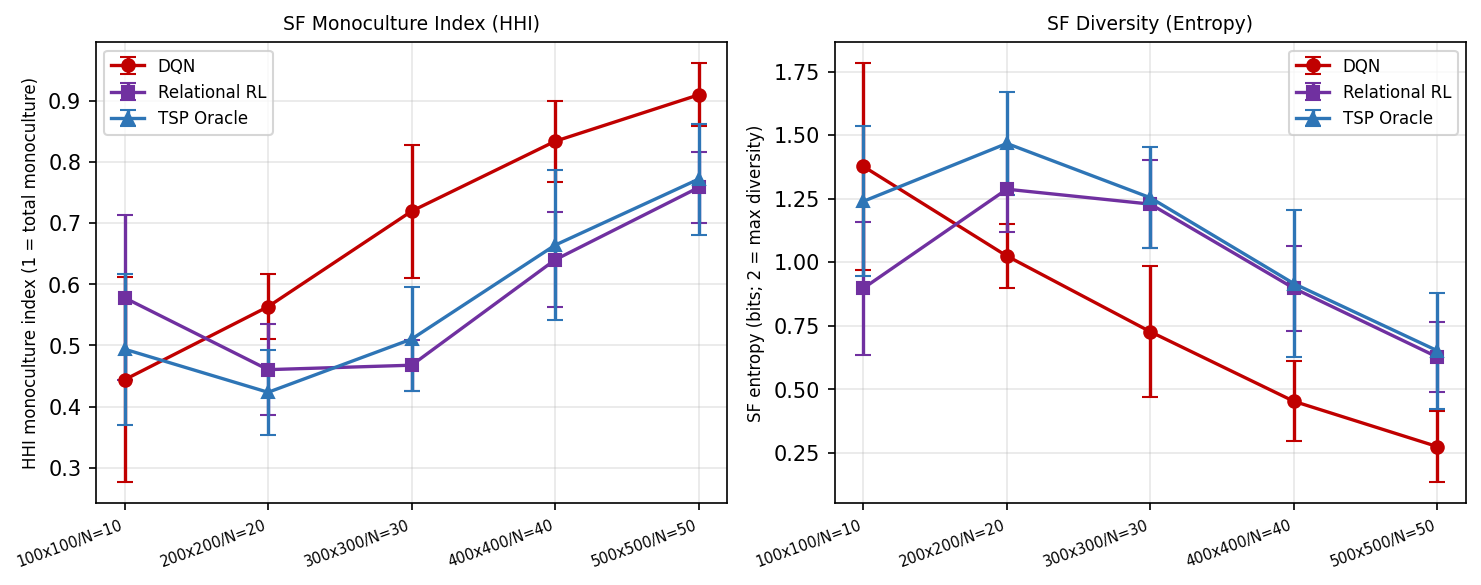
\includegraphics[width=\columnwidth]{sf_monoculture_entropy}
    \caption{SF monoculture index (HHI, left) and Shannon entropy (bits, right) across five scalability conditions (10 seeds). The DQN's perimeter patrol drives sensors toward SF12 monoculture at large scale while triggering zero ADR re-assignments. The Relational RL and TSP Oracle converge to near-identical SF diversity profiles, confirming the architecture fix also restores the protocol benefit.}
    \label{fig:sf_hhi}
\end{figure}

\paragraph{DQN triggers zero ADR events.}
The DQN produces a mean of 0.0 ADR SF changes per sensor across all five conditions. Because the agent patrols the perimeter, its distance to interior sensors is nearly constant throughout each episode. The EMA-RSSI of those sensors never shifts enough to cross an ADR threshold, so they remain locked on whichever SF they were initialised with. At $500{\times}500$/$N{=}50$, 95\% of sensors end the episode on SF12 (HHI $= 0.91$), the slowest and most channel-time-intensive setting---precisely the SF Monoculture the UAV gateway is meant to prevent.

\paragraph{Architecture change restores SF diversity.}
The Relational RL agent triggers 16--105 ADR re-assignments per sensor depending on condition, because it enters the grid interior and varies its distance to sensors. At $300{\times}300$/$N{=}30$ the DQN HHI is 0.72 (entropy 0.73 bits) while the Relational RL reaches HHI $= 0.47$ (entropy 1.23 bits), a diversity gain of 0.50 bits from the architecture change alone. At $N{\ge}40$, the Relational RL and TSP Oracle converge to nearly identical SF profiles (HHI $= 0.76$ vs $0.77$ at $N{=}50$), confirming that interior exploration---not perfect routing---is sufficient to recover near-optimal protocol behaviour. The DQN--Relational RL HHI gap grows monotonically from 0 at $N{=}10$ to $0.15$ at $N{=}50$ (Fig.~\ref{fig:sf_hhi}), tracking the same scale at which NDR diverges.

% ============================================================
\section{Discussion}
% ============================================================

The flat MLP representation is the bottleneck, not the training regime or the reward. Both agents use the same DR/CL schedule, the same reward, and comparable parameter counts. The only difference is that sensor features enter the MLP at positions tied to array index, while they enter the attention module as content-addressed tokens. That change alone recovers 45 percentage points of NDR at $300{\times}300$/30~sensors.

A DQN ablation comparing Domain Randomisation on versus off (20~seeds, fixed $500{\times}500$/$N{=}20$ test condition) shows large-effect advantages for the DR-trained model: Cohen's $d{=}1.43$ on cumulative reward ($p{<}0.001$) and $d{=}1.23$ on Jain's fairness ($p{<}0.001$). This confirms that DR is not redundant even when the architecture is the bottleneck: removing it collapses the DQN faster on out-of-distribution sensor layouts.

There is a fairness gap at $300{\times}300$/30~sensors: Relational RL achieves $J{=}0.564$ vs.\ the TSP Oracle's $J{=}0.819$. This reflects different objectives, not different capabilities. The Oracle runs a uniform spatial tour; the Relational agent optimises urgency-weighted collection and sometimes skips low-urgency sensors to serve overflowing buffers first. Adding an explicit fairness constraint~\cite{jain1984quantitative,lee2025quasi,nemer2022energyefficient} to the Relational RL objective is a direct next step.

At $500{\times}500$/50~sensors the Relational agent reaches 56.4\% NDR vs.\ the Oracle's 76.8\%. This 20~pp gap is physical: the 274~Wh battery is not sufficient to visit all 50~sensors across a 500~m grid in 2100~steps. The agent is at the battery constraint, not a policy ceiling. Multi-UAV coordination~\cite{lee2025quasi,ahmed2026marl,bayerlein2020uav} is the straightforward extension for this density regime.

The Capture Effect adds a spatial optimisation that neither greedy baseline solves optimally. At small scale (SF7 regime) co-SF collisions are rare and greedy achieves $J{\approx}1.0$. At $300{\times}300$/30~sensors, where multiple sensors share SF11 or SF12, the Relational agent positions itself for a 6~dB SINR advantage over co-SF interferers, yielding both higher throughput and lower AoI than the SF-Aware Greedy.

% ============================================================
\section{Conclusion}
% ============================================================

A DQN with Domain Randomisation and Curriculum Learning works at small scale but fails at larger conditions because the flat MLP input encodes sensor features at fixed array positions, making the policy permutation-dependent. At $300{\times}300$~m with 30~sensors the trained DQN reaches only 52.7\% sensor coverage, 32~pp below the SF-Aware Greedy. Replacing the flat MLP with a cross-attention module produces a policy that is permutation-invariant by construction. The Relational RL agent trained with PPO on the same curriculum reaches 97.7\% coverage at $300{\times}300$/30~sensors ($+45$~pp over the DQN, $+13.4$~pp over the best greedy, $p{<}0.001$) and leads all non-oracle agents at every tested condition. Against a TSP Oracle upper bound the Relational agent recovers 73--98\% of oracle coverage at moderate scale; the remaining gap at large scale is the battery budget.

Future work: multi-UAV coordination~\cite{lee2025quasi,ahmed2026marl}; stateful temporal modelling with GTrXL~\cite{parisotto2020gtrxl}; joint fairness-constrained attention toward 6G IoT densities~\cite{nguyen20226g}; and hardware-in-the-loop validation to quantify the sim-to-real gap~\cite{zhao2021sim2real}.

\section*{Acknowledgment}
The author thanks Dr.\ Zahra Mobini for supervision throughout this project.

% ============================================================
\begin{thebibliography}{00}

\bibitem{wei2022uav}
Z. Wei, Z. Feng, Q. Zhang, and W. Xu,
``{UAV}-assisted data collection for internet of things: A survey,''
\textit{IEEE Internet of Things J.}, vol.~9, no.~17, pp.~15460--15483, 2022.

\bibitem{mnih2015humanlevel}
V. Mnih \textit{et al.},
``Human-level control through deep reinforcement learning,''
\textit{Nature}, vol.~518, no.~7540, pp.~529--533, 2015.

\bibitem{zorbas2025revisiting}
D. Zorbas, A. Sabyrbek, and L. Di Puglia Pugliese,
``Revisiting the problem of optimizing spreading factor allocations
in {LoRaWAN}: From theory to practice,''
\textit{Comput. Commun.}, vol.~243, p.~108321, 2025.

\bibitem{xiong2023flyinglora}
R. Xiong \textit{et al.},
``{FlyingLoRa}: Towards energy efficient data collection
in {UAV}-assisted {LoRa} networks,''
\textit{Comput. Netw.}, vol.~220, p.~109511, 2023.

\bibitem{nguyen20226g}
D. C. Nguyen \textit{et al.},
``{6G} internet of things: A comprehensive survey,''
\textit{IEEE Internet of Things J.}, vol.~9, no.~1, pp.~359--383, 2022.

\bibitem{lee2025quasi}
S. Lee, T.-W. Ban, and H. Lee,
``Network-wide energy-efficiency maximization in {UAV}-aided {IoT} networks:
Quasi-distributed deep reinforcement learning approach,''
\textit{IEEE Internet of Things J.}, vol.~12, no.~11,
pp.~15404--15414, 2025.

\bibitem{zhang2021energy}
L. Zhang, A. Celik, S. Dang, and B. Shihada,
``Energy-efficient trajectory optimization for {UAV}-assisted {IoT} networks,''
\textit{IEEE Trans. Mobile Comput.}, vol.~21, no.~8,
pp.~2869--2883, 2022.

\bibitem{bengio2009curriculum}
Y. Bengio, J. Louradour, R. Collobert, and J. Weston,
``Curriculum learning,''
in \textit{Proc. ICML}, 2009, pp.~41--48.

\bibitem{tobin2017domain}
J. Tobin \textit{et al.},
``Domain randomization for transferring deep neural networks from simulation
to the real world,''
in \textit{Proc. IEEE/RSJ IROS}, 2017, pp.~23--30.

\bibitem{towers2024gymnasium}
M. Towers \textit{et al.},
``Gymnasium: A standard interface for reinforcement learning environments,''
arXiv:2407.17032, 2024.

\bibitem{kaul2012realtime}
S. Kaul, R. Yates, and M. Gruteser,
``Real-time status: How often should one update?''
in \textit{Proc. IEEE INFOCOM}, 2012, pp.~2731--2735.

\bibitem{abdelmagid2019aoi}
M. A. Abd-Elmagid, N. Pappas, and H. S. Dhillon,
``On the role of age of information in the internet of things,''
\textit{IEEE Commun. Mag.}, vol.~57, no.~12, pp.~72--77, 2019.

\bibitem{challita2018interference}
U. Challita, W. Saad, and C. Bettstetter,
``Deep reinforcement learning for interference-aware path planning
of cellular-connected {UAVs},''
in \textit{Proc. IEEE ICC}, 2018.

\bibitem{croce2020lora}
D. Croce \textit{et al.},
``{LoRa} technology demystified: From link behavior to cell-level performance,''
\textit{IEEE Trans. Wireless Commun.}, vol.~19, no.~2, pp.~822--834, 2020.

\bibitem{zeng2017energy}
Y. Zeng and R. Zhang,
``Energy-efficient {UAV} communication with trajectory optimization,''
\textit{IEEE Trans. Wireless Commun.}, vol.~16, no.~6, pp.~3747--3760, 2017.

\bibitem{zambaldi2018relational}
V. Zambaldi \textit{et al.},
``Relational deep reinforcement learning,''
arXiv:1806.01830, 2018.

\bibitem{schulman2017proximal}
J. Schulman, F. Wolski, P. Dhariwal, A. Radford, and O. Klimov,
``Proximal policy optimization algorithms,''
arXiv:1707.06347, 2017.

\bibitem{vaswani2017attention}
A. Vaswani \textit{et al.},
``Attention is all you need,''
in \textit{Proc. NeurIPS}, 2017, pp.~5998--6008.

\bibitem{luong2019drl}
N. C. Luong \textit{et al.},
``Applications of deep reinforcement learning in communications
and networking: A survey,''
\textit{IEEE Commun. Surveys Tuts.}, vol.~21, no.~4,
pp.~3133--3174, 2019.

\bibitem{raffin2021stable}
A. Raffin \textit{et al.},
``Stable-{Baselines3}: Reliable reinforcement learning implementations,''
\textit{J. Mach. Learn. Res.}, vol.~22, no.~268, pp.~1--8, 2021.

\bibitem{bayerlein2020uav}
H. Bayerlein, M. Theile, M. Caccamo, and D. Gesbert,
``{UAV} path planning for wireless data harvesting:
A deep reinforcement learning approach,''
arXiv:2007.00544, 2020.

\bibitem{zeng2016wireless}
Y. Zeng, R. Zhang, and T. J. Lim,
``Wireless communications with unmanned aerial vehicles:
Opportunities and challenges,''
\textit{IEEE Commun. Mag.}, vol.~54, no.~5, pp.~36--42, 2016.

\bibitem{mozaffari2019tutorial}
M. Mozaffari, W. Saad, M. Bennis, Y.-H. Nam, and M. Debbah,
``A tutorial on {UAVs} for wireless networks: Applications,
challenges, and open problems,''
\textit{IEEE Commun. Surveys Tuts.}, vol.~21, no.~3,
pp.~2334--2360, 2019.

\bibitem{bor2016lora}
M. Bor, J. E. Vidler, and U. Roedig,
``{LoRa} for the internet of things,''
in \textit{Proc. EWSN}, 2016, pp.~361--366.

\bibitem{augustin2016lora}
A. Augustin, J. Yi, T. Clausen, and W. M. Townsley,
``A study of {LoRa}: Long range and low power networks
for the internet of things,''
\textit{Sensors}, vol.~16, no.~9, p.~1466, 2016.

\bibitem{slabicki2018adaptive}
M. Slabicki, G. Premsankar, and M. Di Francesco,
``Adaptive configuration of {LoRa} networks for dense {IoT} deployments,''
in \textit{Proc. IEEE/IFIP NOMS}, 2018.

\bibitem{jain1984quantitative}
R. Jain, D.-M. Chiu, and W. Hawe,
``A quantitative measure of fairness and discrimination
for resource allocation in shared computer systems,''
DEC Tech. Rep. DEC-TR-301, 1984.

\bibitem{rappaport2002wireless}
T. S. Rappaport,
\textit{Wireless Communications: Principles and Practice}, 2nd~ed.
Prentice Hall, 2002.

\bibitem{zaheer2017deepsets}
M. Zaheer \textit{et al.},
``Deep sets,''
in \textit{Proc. NeurIPS}, vol.~30, 2017.

\bibitem{kool2019attention}
W. Kool, H. van Hoof, and M. Welling,
``Attention, learn to solve routing problems!''
in \textit{Proc. ICLR}, 2019.

\bibitem{alhourani2014optimal}
A. Al-Hourani, S. Kandeepan, and S. Lardner,
``Optimal {LAP} altitude for maximum coverage,''
\textit{IEEE Wireless Commun. Lett.}, vol.~3, no.~6,
pp.~569--572, 2014.

\bibitem{nemer2022energyefficient}
I. A. Nemer \textit{et al.},
``Energy-efficient {UAV} movement control for fair communication
coverage: A deep reinforcement learning approach,''
\textit{Sensors}, vol.~22, no.~5, p.~1919, 2022.

\bibitem{liu2019uav}
C. H. Liu \textit{et al.},
``Energy-efficient {UAV} control for effective and fair communication
coverage: A deep reinforcement learning approach,''
\textit{IEEE J. Sel. Areas Commun.}, vol.~36, no.~9,
pp.~2059--2070, 2018.

\bibitem{lin1973tsp}
S. Lin and B. W. Kernighan,
``An effective heuristic algorithm for the traveling-salesman problem,''
\textit{Oper. Res.}, vol.~21, no.~2, pp.~498--516, 1973.

\bibitem{openai2019dexterous}
{OpenAI} \textit{et al.},
``Learning dexterous in-hand manipulation,''
\textit{Int. J. Robot. Res.}, vol.~39, no.~1, pp.~3--20, 2020.

\bibitem{zhao2021sim2real}
W. Zhao, J. P. Queralta, and T. Westerlund,
``Sim-to-real transfer in deep reinforcement learning for robotics:
A survey,''
arXiv:2009.13303, 2021.

\bibitem{matiisen2017teacher}
T. Matiisen, A. Oliver, T. Cohen, and J. Schulman,
``Teacher-student curriculum learning,''
\textit{IEEE Trans. Neural Netw. Learn. Syst.}, vol.~31, no.~9,
pp.~3732--3742, 2020.

\bibitem{tripathi2022aoi}
V. Tripathi and E. Modiano,
``Optimizing age of information with correlated sources,''
in \textit{Proc. ACM MobiHoc}, 2022.

\bibitem{cappart2023combinatorial}
Q. Cappart \textit{et al.},
``Combinatorial optimization and reasoning with graph neural networks,''
\textit{J. Mach. Learn. Res.}, vol.~24, no.~130, pp.~1--61, 2023.

\bibitem{li2020uav}
B. Li, Z. Fei, and Y. Zhang,
``{UAV} communications for 5{G} and beyond:
Recent advances and future trends,''
\textit{IEEE Internet of Things J.}, vol.~6, no.~2,
pp.~2241--2263, 2019.

\bibitem{schulman2016gae}
J. Schulman, P. Moritz, S. Levine, M. Jordan, and P. Abbeel,
``High-dimensional continuous control using generalized advantage estimation,''
in \textit{Proc. ICLR}, 2016.

\bibitem{parisotto2020gtrxl}
E. Parisotto \textit{et al.},
``Stabilizing transformers for reinforcement learning,''
in \textit{Proc. ICML}, 2020.

\bibitem{reynders2016range}
B. Reynders, W. Meert, and S. Pollin,
``Range and coexistence analysis of long range unlicensed communication,''
in \textit{Proc. IEEE ICT}, 2016.

\bibitem{chen2021decision}
L. Chen \textit{et al.},
``Decision transformer: Reinforcement learning via sequence modeling,''
in \textit{Proc. NeurIPS}, 2021.

\bibitem{semtech2020sx1276}
{Semtech Corporation},
``{SX1276/77/78/79} datasheet: 137~{MHz} to 1020~{MHz} low power long range transceiver,''
Rev.~7, 2020.

\bibitem{ahmed2026marl}
A. I. Ahmed, J. Bentahar, and E. M. Amhoud,
``Energy-efficient {UAV}-assisted {LoRa} gateways:
A multi-agent optimization approach,''
in \textit{Proc. IEEE VTC2026-Spring}, 2026.

\end{thebibliography}

\end{document}
